\documentclass[reprint,english,notitlepage]{revtex4-2}
\usepackage{amsmath}
\usepackage[mathletters]{ucs}
\usepackage[utf8x]{inputenc}
\usepackage[english]{babel}
\usepackage{esint}
\usepackage{physics,amssymb}
\usepackage{graphicx}
\usepackage{xcolor}
\usepackage{hyperref}
\usepackage{listings}
\usepackage{subfigure}
\usepackage[style=science, backend=biber]{biblatex}
\addbibresource{Report_Part_9.bib}
\hypersetup{
    colorlinks,
    linkcolor={red!50!black},
    citecolor={blue!50!black},
    urlcolor={blue!80!black}}

\lstset{inputpath=,
    backgroundcolor=\color{white!88!black},
    basicstyle={\ttfamily\scriptsize},
    commentstyle=\color{magenta},
    language=Python,
    morekeywords={True,False},
    tabsize=4,
    stringstyle=\color{green!55!black},
    frame=single,
    keywordstyle=\color{blue},
    showstringspaces=false,
    columns=fullflexible,
    keepspaces=true}

\begin{document}

\title{Interplanetary Rocket Launch}
\author{Candidates: 15369 \& 15401}
\date{\today}
\affiliation{Institute of Theoretical Astrophysics, University of Oslo}

\maketitle

\section{Exercise 1}\label{sec:exercise-1}
    \subsection{Introduction}\label{subsec:introduction1}
        In this exercise, we will be looking at the gravitational Doppler shift when taking General Relativity into account.
        As the name might give away, General Relativity is the generalization of the theory of Special Relativity.
        This theory describes spacetime as a four-dimensional geometry with three spatial dimensions and one time dimension.
        In General Relativity, gravity is described as a deformation in spacetime geometry and is directly related to the momentum, energy and mass of the present objects.~\parencite[][]{wiki_gr}
        This is an effect, where the gravitational deformation of spacetime affects the wavelength of light, so that it appears either longer or shorter.\\
        For an observer close to a large mass, the mass will deform spacetime in a way, so that time moves at a different rate than for a far-away observer.
        This time difference, affects the frequency and therefore wavelength of light that is sent out from the observer close to the mass.
        We will try to describe this difference in wavelength for an observer close to the mass and the observer far away as it affects how we observe light from other objects in the universe.

    \subsection{Situation}\label{subsec:situation1}
        We will be looking at our own solar system containing the sun and the earth.
        To simplify things, we will be using polar coordinates.\\
        One observer will be positioned on the surface of the sun using so-called shell coordinates, whereas another observer will be positioned far away from the sun.
        Shell coordinates are the local coordinates for the shell observer.
        For such a shell observer stationed outside the Schwarzschild radius of an object, spacetime is not as deformed as inside the Schwarzschild radius.
        We are therefore able to use special relativity for minuscule intervals $\Delta t$ and $\Delta r$.
        This allows us to measure the wavelength of the light perceived by both observers.\\
        We will then send out light, or electromagnetic waves, radially outward from the mass or inwards to the mass.
        This way, we are able to simplify our calculations and neglect tangential components.

    \subsection{Method}\label{subsec:method1}
        According to general relativity, the time interval $\Delta t_{shell}$ between the two peaks of the electromagnetic wave varies when spacetime is deformed, such as in the presence of a large mass.\\
        To be able to relate the time intervals $\Delta t$, which is the time interval seen by an observer far away, and $\Delta t_{shell}$, which is the time interval for the shell observer, we will be using the formula for the Schwarzschild line element (which can be found in ~\parencite[][]{lecture2c}) between two ticks $A$ and $B$ on the clock of the shell observer.\\

        By using the fact that the shell observer is at rest, the equation for the Schwarzschild line element can be simplified, and $\Delta s_{AB}$ can be substituted by $\Delta t_{shell}$.
        This yields the formula
        \begin{align}
                \Delta t = \frac{\Delta t_{shell}}{\sqrt{\left(1-\frac{2M}{r}\right)}} \label{eq2}
        \end{align}
        The derivation of this formula can be found in section ~\ref{subsec:derivation-of-time-interval-difference}\\\\

        This formula for the difference in time intervals for the observers, can then be used to find the gravitational Doppler shift of light, which is close to a large mass.
        We know that the Doppler shift is given by formula~\eqref{grav_dopplershift1}.
        \begin{align}
            \frac{\Delta \lambda}{\lambda_{shell}} \label{grav_dopplershift1}
        \end{align}
        Since we define the relationship of the frequency $\nu$ and the wavelength $\lambda$ to be $\nu = \frac{c}{\lambda}$ and $\nu = \frac{1}{\Delta t}$, we can substitute $\lambda$ by $\Delta_t$ and $\lambda_{shell}$ by $\Delta_t_{shell}$ in equation ~\eqref{grav_dopplershift1}.
        By then inserting the expression found in ~\eqref{eq2}, we get
        \begin{align}
            \frac{\Delta \lambda}{\lambda_{shell}} &= \frac{1}{\sqrt{\left(1-\frac{2M}{r}\right)}} - 1 \label{doppler_shift}
        \end{align}\\\\

        We can see that if the distance $r \gg 2M$, the second term under the root, will be going towards zero.
        We define $x = \frac{2M}{r}$ and create a Taylor expansion around $x = 0$.
        Using a Taylor expansion of degree 1, we find that the Doppler shift can be approximated by
        \begin{align}
            \frac{\Delta \lambda}{\lambda_{shell}} = \frac{M}{r} \label{doppler_shift1}
        \end{align}
        For the derivation, see section~\ref{subsec:exercise-1.3}.
        


    \subsection{Conclusion}\label{subsec:conclusion1}
        Looking at the results, we can see that there are significant effects from general relativity when we are close to a large mass.\\
        By using electromagnetic radiation, we determined the difference in proper time for the observer close to the mass and the far-away observer, and its effects.\\

        When sending electromagnetic radiation radially outwards from the mass, the wavelength of the radiation, will appear increased for a far-away observer or redshifted.
        The opposite effect happens when radiation is sent inwards to the mass, which is called blueshift.
        The magnitude of this effect depends on the mass and the radius from where the radiation is sent out or received.
        It can in general be described using formula~\eqref{doppler_shift} and using~\eqref{doppler_shift1} for $r \gg 2M$.




\section{Exercise 2}\label{sec:exercise-2}
    \subsection{Introduction}\label{subsec:introduction2}
        To get a better grasp of the movement of an object when taking general relativity into account, we will be taking a closer look at the Schwarzschild line element.
        Together with the principle of maximum aging, we will be able to derive a quantity, which is equivalent to mechanical spin.\\
        This helps us to further understand movement, and the calculations of the movement in free float.

    \subsection{Situation}\label{subsec:situation2}
        The main object of interest in this exercise is an object, which is orbiting around a black hole with mass $M$ and radius $2M$.
        The orbit does not need to be a circular orbit, but can have an elliptical shape.\\
        We define three points along the orbit of the object (Note that we will be using a polar coordinate system in this exercise).
        Point $1$ at time $t_1$ and position $(r_1, \phi_1)$, point $2$ at time $t_2$ and position $(r_2, \phi_2)$ and point $3$ at time $t_3$ and position $(r_3, \phi_3)$.
        We assume all parameters to be known, except $\phi_2$, and can then define two time steps $\Delta t_{12} = (t_2-t_1)$ and $\Delta t_{23} = (t_3-t_2)$.\\

        In the following derivations and calculations, the time steps $\Delta t_{12}$ and $\Delta t_{23}$ are extremely small, which will allow us to use Lorentz-transformation together with the Schwarzschild line element.
        As the timesteps are so small, we will assume the radius during each interval to be constant and equal to respectively $r_A$ and $r_B$.\\

        The proper time interval corresponding to $\Delta t_{12}$ and $\Delta t_{23}$ are $\Delta\tau_{12}$ and $\Delta\tau_{23}$.

    \subsection{Method}\label{subsec:method2}
        The change in position corresponding to free float is found when minimising the change in spatial coordinates, and therefore maximising the change in time coordinates.
        This is called the principle of maximum aging.
        Finding these changes in coordinates, is a relatively straight forward, but requires some calculations.
        We will first need to approximate $\Delta s_{12}$ and $\Delta s_{23}$ by $\Delta \tau_{12}$ and $\Delta \tau_{23}$.
        This approximation is possible due to the assumption that the radius $r$ is constant during each time interval.\\

        At this point we can define a new time interval $\Delta \tau_{13}$ from point 1 to 3, which is equal to the sum of $\Delta \tau_{12}$ and $\Delta\tau_{23}$.
        The Schwarzschild line element for this new interval, is therefore equal to the sum of the line elements of the other intervals.\\

        By finding the derivative of the line element for $\Delta \tau_{13}$ with respect to $\phi$ and setting it equal to 0, we can find the change in coordinates, which maximizes the change of time coordinates.

    \subsection{Conclusion}\label{subsec:conclusion2}
        When doing the calculations, the terms not including $\phi$ will be constant.
        We now find that the quantity $r^2 \frac{d\phi}{d\tau}$ is the same in both time intervals, even with $d\phi$ and $d\tau$ changing.
        We can therefore conclude that this quantity must be conserved.

        This is an important result, as it tells us that the principle of maximum aging describes a path where the spin is constant.
        When in free fall, an object will therefore move on such a trajectory.\\

        This quantity can be compared to the spin in classical mechanics.
        In classical mechanics, spin is conserved if no outer force is applied, which corresponds to the trajectory of the object in free fall.




\section{Exercise 6}\label{sec:exercise-6}
    \subsection{Introduction}\label{subsec:introduction6}
        Since the mass of a black hole is so large, that it even attracts light and nothing can escape from it, they are very intimidating.
        However, as long as we are not inside the event horizon, objects tend to behave just like in the presence of an extremely heavy and dense star.\\
        This begs the question: What happens if we accidentally set a course very close to, or even into a black hole?
        And what happens if we are being pulled inside the black hole?\\
        The answer to this question is connected to Energy, and potential.
        This relativistic energy and potential are very similar, but not identical to the ones from classical mechanics.


    \subsection{Situation}\label{subsec:situation6}
        The system we will be using to determine the fate of an object floating towards a black hole, will be containing a black hole in the center of our polar coordinate system with a mass M.\\
        We now have a rocket at a shell-coordinate around the black hole with radius 20M.
        The rocket is flying with a velocity of $v_{shell} = 0.993c$ at an angle of $\phi = 167^{\circ}$ (measured from the radial vector).
        However, at this point, the engines break, which means the rocket will now be floating freely until the engines are fixed.
        The situation can be seen in figure~\ref{fig:setup6}.

        \begin{figure}[h]
            \centering
            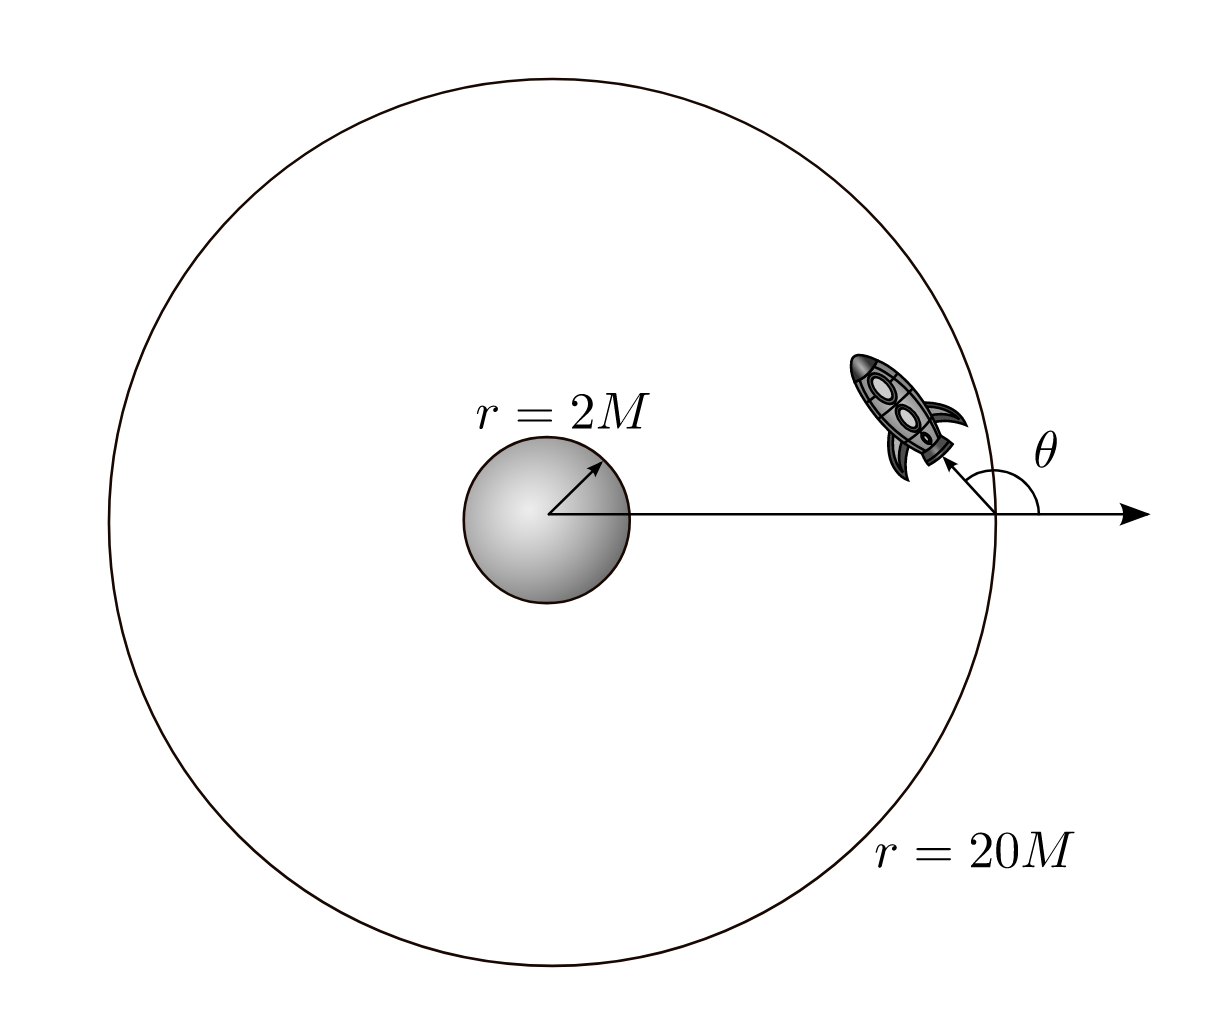
\includegraphics[scale=0.3]{setup6}
            \caption{A graphical depiction of the situation in exercise 6. From~\parencite[][page 6]{part9}}\label{fig:setup6}
        \end{figure}


    \subsection{Method}\label{subsec:method6}
        After the engine failure the rocket is floating freely, which means we will be able to perform some calculations for its trajectory.
        For a rocket on a trajectory towards a black hole, there are generally three outcomes.
        The rocket can either continue orbiting around the black hole, fall into the black hole or escape from its gravitational pull.\\

        To determine the outcome, we will be calculating the potential of the rocket when it's getting closer to the black hole.
        The potential consists of both kinetic potential and gravitational potential.
        A graph of this potential might therefore look something like figure~\ref{fig:potential_sketch}.

        \begin{figure}[h]
            \centering
            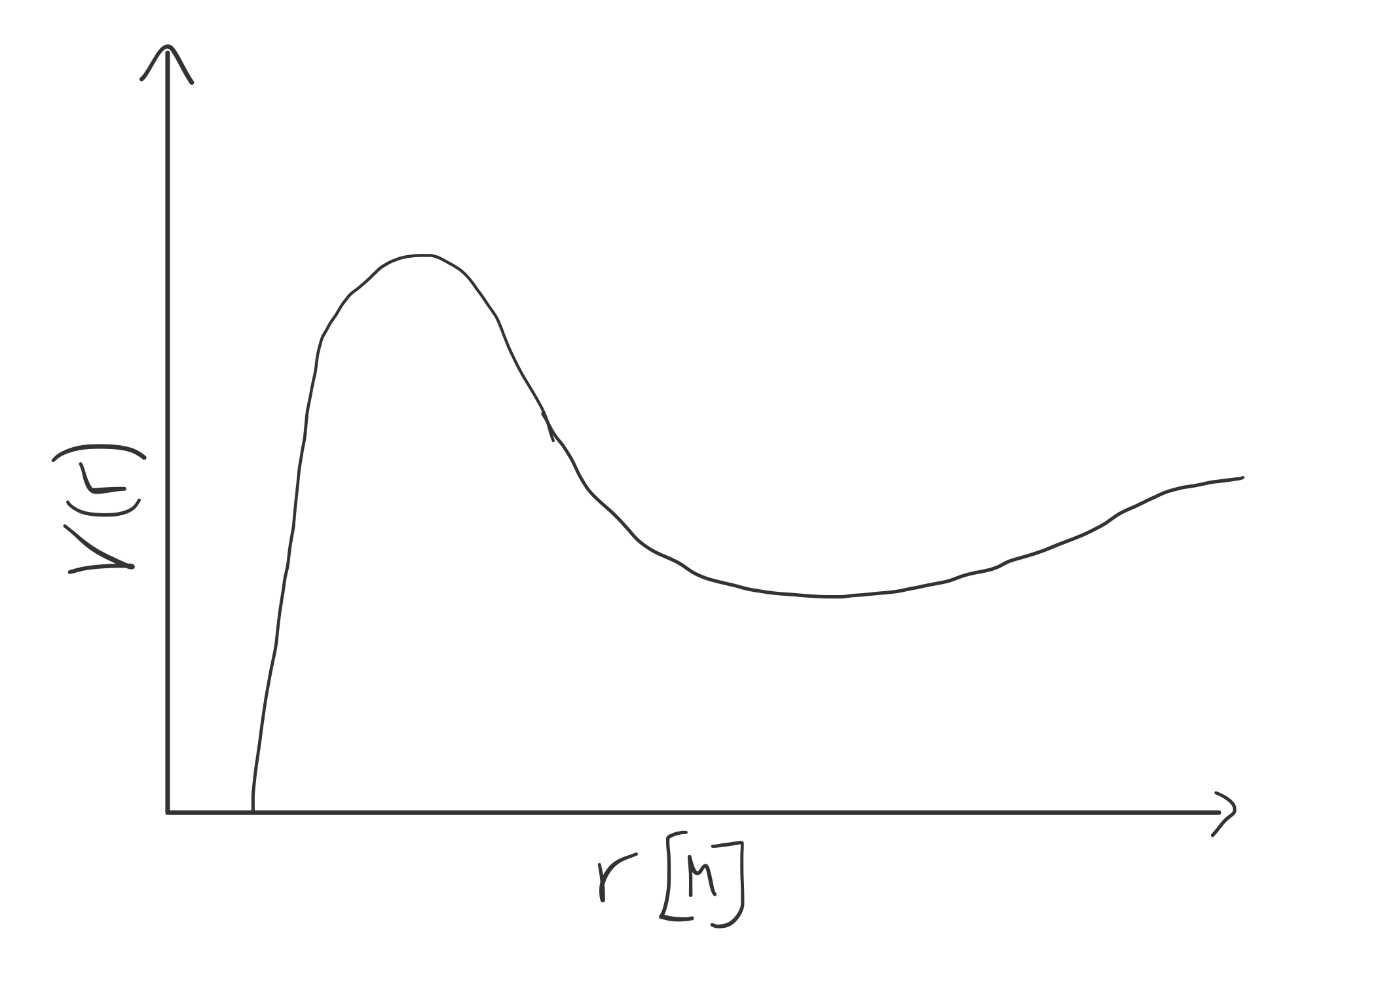
\includegraphics[scale=0.15]{potential_sketch}
            \caption{A sketch of the potential of an object around a black hole as a function of radius.}\label{fig:potential_sketch}
        \end{figure}

        Furthermore, we will have to look at the energy of the rocket, as this will determine its fate.
        The potential is given by formula~\eqref{eq_potential}.
        \begin{align}
            V(r) = \sqrt{\left( 1- \frac{2M}{r}\right) \left[1 + \frac{\left(L/m \right)^2}{r^2}}\right]_{}^{} \label{eq_potential}
        \end{align}

        When looking at the effective potential for an object around a black hole in figure~\ref{fig:potential_sketch}, we see that a rocket falling towards the black hole will first lose some potential.
        Thereafter, it gains potential very quickly, before losing it rapidly again after crossing the critical radius $r_{crit}$ and falling into the black hole.\\
        To fall into the black hole, the rocket therefore needs enough energy, which can be converted to potential energy to overcome this "hill" in potential.
        This amount of energy at the radius $r_{crit}$ is called the critical energy per mass $\frac{E_{crit}}{m}$ of the black hole.\\

        By calculating the Energy per mass of the rocket $\frac{E}{m}$ using formula~\eqref{energy_per_mass} and comparing it to the critical energy per mass $\frac{E_{crit}}{m}$, we can determine the fate of the rocket.
        \begin{align}
            \frac{E}{m} = \sqrt{1-\frac{2M}{R}}\gamma_{shell} \label{energy_per_mass}
        \end{align}





    \subsection{Conclusion}\label{subsec:conclusion6}
        We find that there are three outcomes to this tricky situation.
        According to our calculations, the fate of the rocket is dependent on the total energy per mass of the rocket and the critical energy of the black hole.\\

        If the total energy per mass of the rocket is less than this critical energy, the rocket will not be able to overcome the "hill" of potential when getting close to the black hole, and therefore not be able to enter the black hole.
        However, if the energy per mass is larger than this critical energy, the rocket will get close enough to the black hole to be pulled inside.\\
        An energy per mass lower than the critical energy per mass will therefore result in the rocket falling back into the "pit" of potential seen in figure~\ref{fig:potential_sketch}.
        From there, the rocket can have two different outcomes.\\
        If the energy is between $\frac{E_{crit}}{m}$ and $\lim_{r \rightarrow \infty} \frac{V(r)}{m}$, the rocket will be able to escape the gravitational pull of the black hole, and the rocket is safe.
        If the energy is lower than $\lim_{r \rightarrow \infty} \frac{V(r)}{m}$ the rocket will be stuck inside the "pit" of potential energy, and end up orbiting the black hole forever (given that we will not be able to fix the engine).\\

        In our case, the energy per mass is higher than the critical energy as seen in figure~\ref{fig:eff_potential}, and the rocket will therefore fall into the black hole.\\

        \begin{figure}[h]
            \centering
            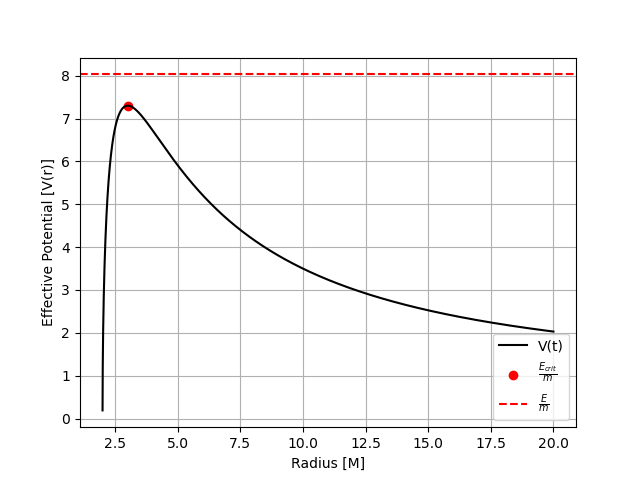
\includegraphics[scale=0.4]{ex6_effpotential}
            \caption{The effective potential as a function of radius around the black hole. The energy per mass of the rocket is seen in red.}\label{fig:eff_potential}
        \end{figure}

        After falling into the black hole, the gravitational forces will be so extreme, and increase so much relative to the radius that different body parts of the astronaut in the rocket will experience different forces.\\
        The part closest to the black hole will experience a much stronger force than the body part furthest from the black hole.\\
        This means the astronaut will be stretched along his length.
        This effect is called Spaghettification, as the astronaut will look like a spaghetti in the end, which can be seen in figure~\ref{fig:spaghettification}.

        \begin{figure}[h]
            \centering
            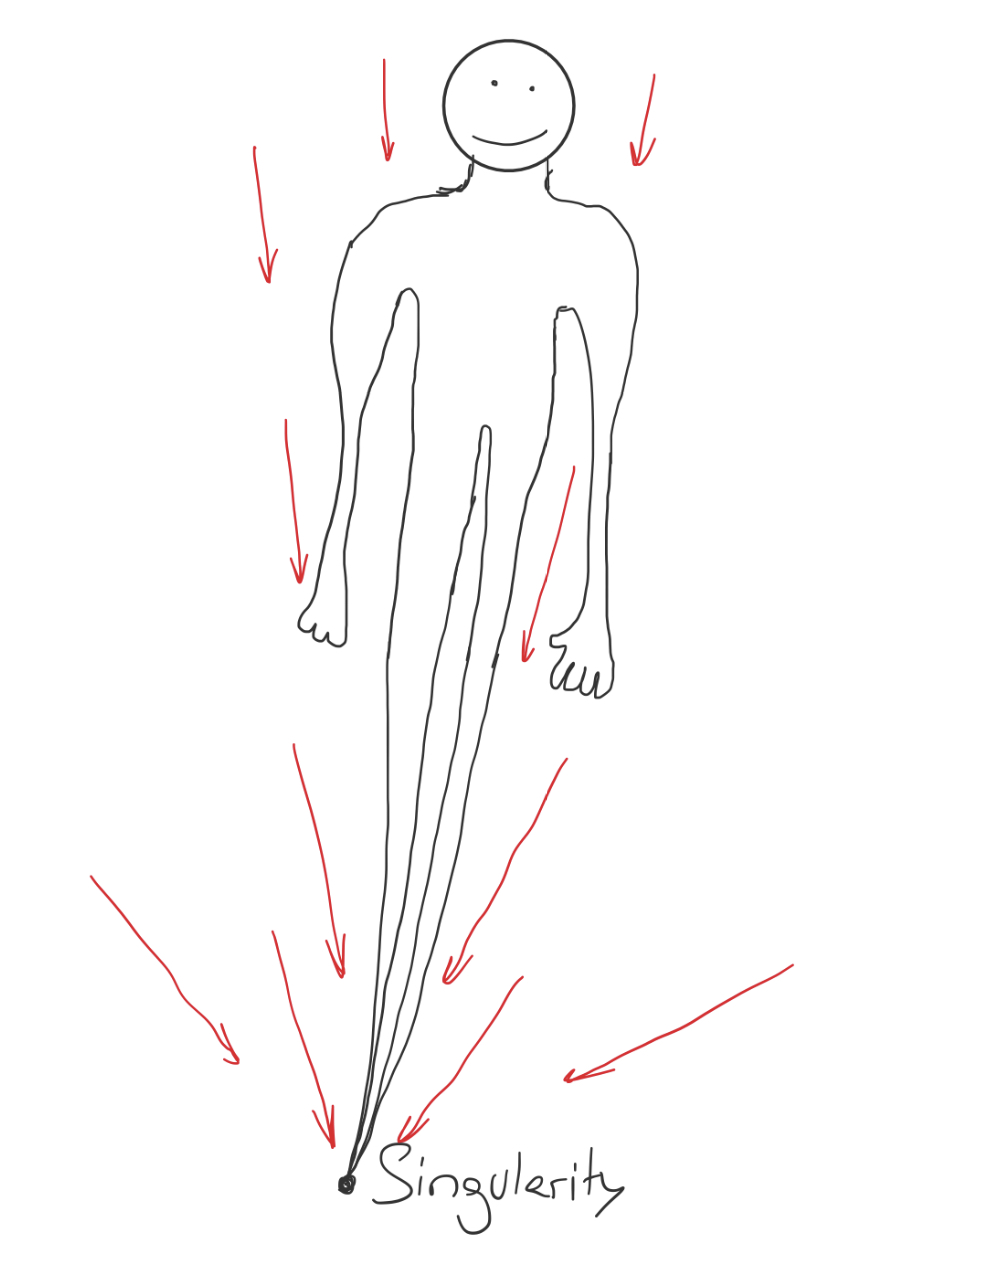
\includegraphics[scale=0.15]{spaghettification}
            \caption{Sketch of the Spaghettification effect and the gravitational forces on the astronaut (red)}\label{fig:spaghettification}
        \end{figure}


\newpage
\section{Exercise 7}\label{sec:exercise-7}
    \subsection{Introduction}\label{subsec:introduction7}
        After entering the event horizon, things get a bit weird.
        The gravitational effects will get so strong that the time and space dimensions switch places.
        Fortunately though, we managed to fix the rocket engine, and able to use it for one last attempt to escape the black hole.\\\\
        However, escaping out of a black hole is just as difficult as one might imagine, and we therefore need to study the environment inside the black hole a bit to plan our attempt.\\
        This involves sending out two beams of light from the rocket.
        One is sent out towards the center of the black hole, and the other radially outwards.
        By studying the behaviour of these light beams, we will be able to evaluate whether our rocket is able to escape.

    \subsection{Situation}\label{subsec:situation7}
        We are still looking at the same black hole as in exercise 6 (\ref{sec:exercise-6}).
        However, this time the rocket with our astronaut has already entered the event horizon and is therefore inside the black hole.
        In other words the rocket is at a radius of $r < 2M$.\\
        The rocket is falling towards the center of the black hole at a velocity, as if the rocket started falling freely from very far away with $v = 0$.\\
        As stated in section~\ref{subsec:introduction7}, we emitted two light beams to examine our environment to determine our chance of escape.
        These light beams are moving radially towards, and away from the black hole.
        This means that for the light beams $d\phi = 0$.
        Furthermore, $d\tau = 0$ as it is for all light beams traveling at the speed of light.

    \subsection{Method}\label{subsec:method7}
        As things are a bit weird inside the black hole, and some mathematics that we use outside the black hole tend to break down, we have measure things a bit differently.\\
        We will not be able to use the Schwarzschild time anymore, since it is meant for the environment outside the black hole.
        Therefore, we want to express the Schwarzschild line element using the wristwatch time of the astronaut instead of the Schwarzschild time.\\
        Luckily, we were able to do this just before entering the black hole.
        We were therefore able to use shell coordinate frames as a tool to do this change of coordinate.\\

        Since the shell observer at these shell coordinates just outside the event horizon is at rest, we can use special relativity and therefore Lorentz transformation to express the wristwatch time in terms of shell coordinates.
        By using the know relations between shell coordinates and Schwarzschild coordinates, as well as an expression for the shell velocity (found in~\parencite[][page 7]{lecture2d}) we can derive a new form of the Schwarzschild line element.\\

        This new form of the Schwarzschild line element can then be used to describe the movement of the light beams inside the black hole.
        Due to the nature of light beams and by emitting them radially, we can use the assumptions from section~\ref{subsec:situation7} to simplify the equation and get~\eqref{velocity_beams}.
        \begin{align}
            \frac{dr}{dt'} = -\sqrt{\frac{2M}{r}} \pm 1 \label{velocity_beams}
        \end{align}

        The plus-minus sign here refers to the two different directions at which the light beams are emitted.\\

        To get a better understanding of the meaning of this equation and the movement of the light we will now to some reasoning.\\
        By examining~\eqref{velocity_beams} closer, we see that for the light beam emitted towards the center of the black hole, the velocity will always be negative since both terms are negative.
        It will move at the speed of light far away from the black hole, and increase its velocity the closer it gets to the event horizon.
        At the event horizon where $r = 2M$, its velocity will be twice the speed of light and will increase with decreasing distance.\\

        For the light beam sent outwards, the velocity will be radially outwards outside the black hole and increase with increasing distance.
        At the event horizon, the velocity will be 0.
        Inside the black hole, the velocity of the light beam sent radially outwards will change direction immediately and move towards the center of the black hole instead.
        Its velocity will increase as the distance to the singularity decreases, but will be less than the velocity of the light beam which has been emitted towards the singularity.


    \subsection{Conclusion}\label{subsec:conclusion7}
        We have now examined the movement of the two light beams and found an expression~\eqref{velocity_beams} for their velocity.
        Their movement is also described in the Minkowski diagram of the rocket~\ref{fig:world_line}, describing the movement of the rocket along its world line.

        \begin{figure}[h]
            \centering
            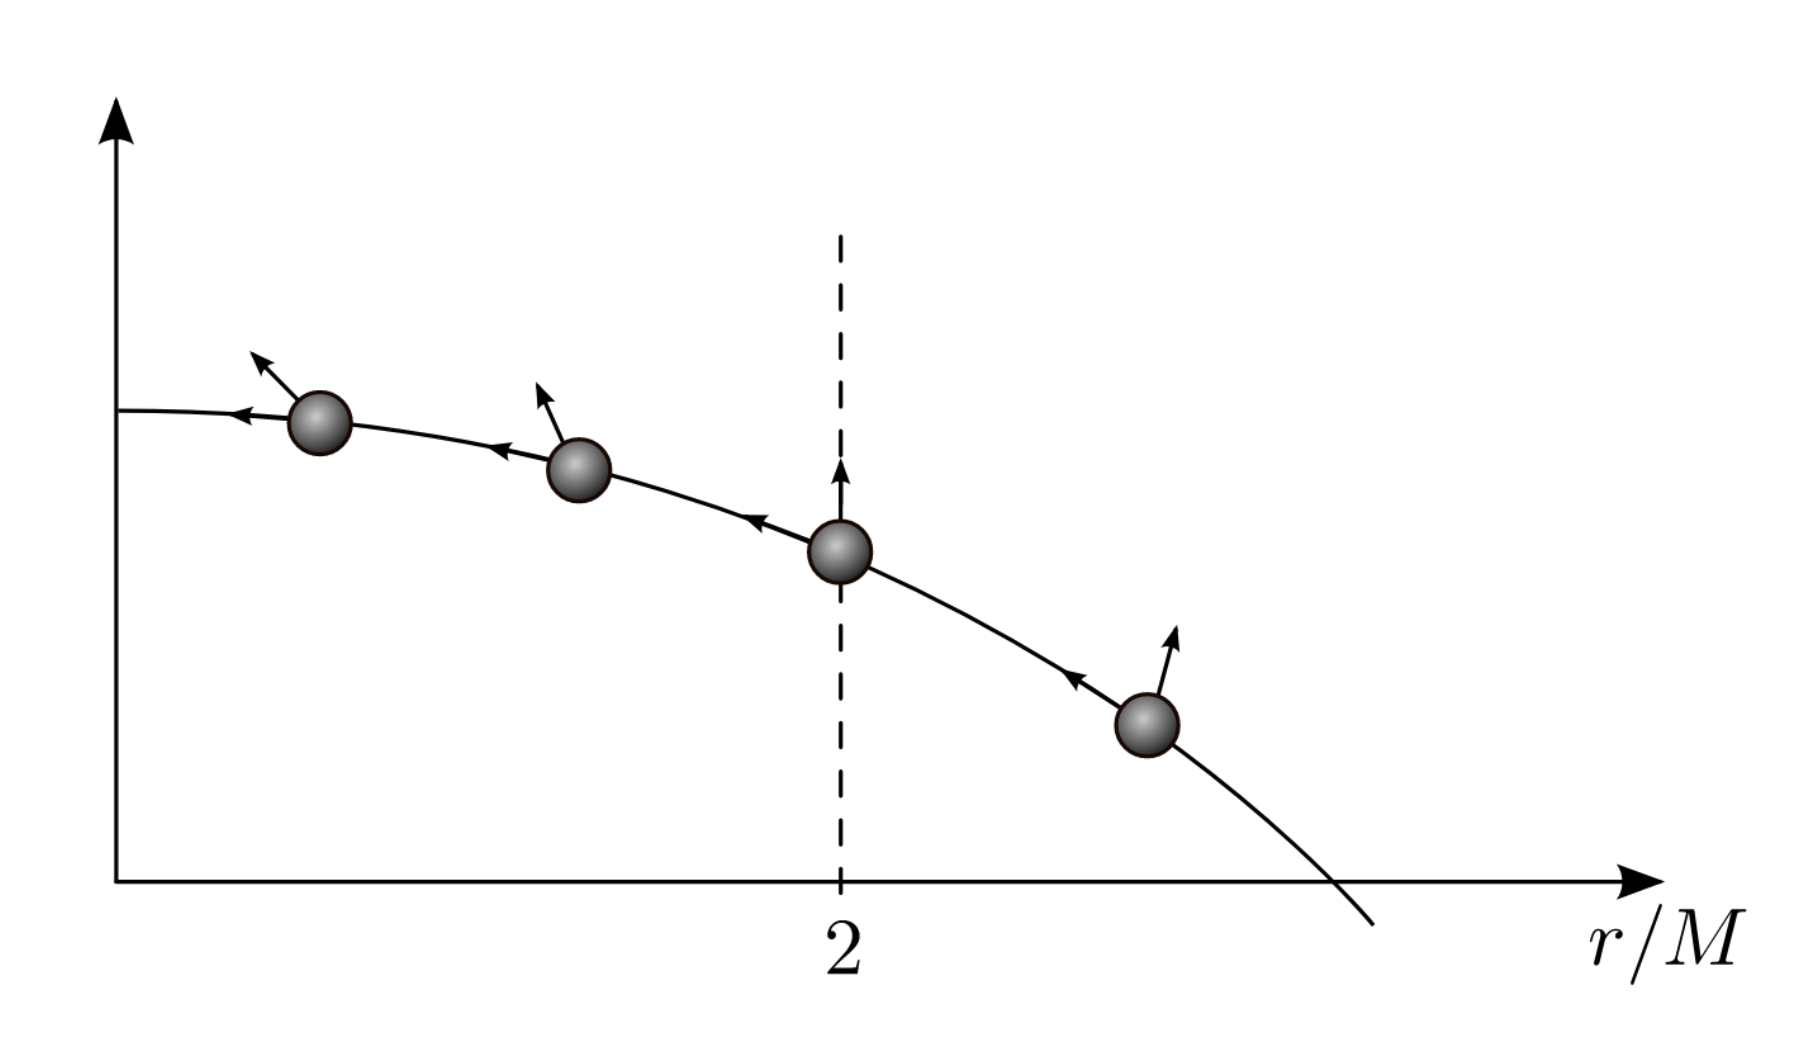
\includegraphics[scale=0.2]{world_line}
            \caption{A Minkowski diagram of the rocket. The position of the rocket is represented by the balls and the light beams by the arrows.}\label{fig:world_line}
        \end{figure}

        We see that the rocket starts by moving in both the time and spatial dimensions.
        The closer it gets to the singularity, the more it accelerates in the spatial dimensions and less it moves in the time dimension.
        When the rocket reaches the singularity, it only moves in the spatial dimension, and not into the time dimension anymore.
        Time has therefore stopped completely for it.\\

        Looking at the arrows, we see a behaviour corresponding to the earlier reasoning of the movement of the light beams.\\
        The light beam which is sent outwards, moves a lot in both the time and spatial dimensions.
        When reaching the event horizon at $r = 2M$, it stops moving in the spatial dimension and only moves in the time dimension, before accelerating towards the singularity in the spatial dimension and correspondingly decreasing its movement in the time dimension.\\
        The light beam, which is emitted radially towards the singularity, always follows the world line of the rocket, as it is being sent out in the same direction.
        Just like the rocket, it moves in both the spatial and time dimensions further away from the singularity, but decreases its movement in the time direction as the radius decreases and the velocity in the spatial dimension increases according to formula~\eqref{velocity_beams}.\\

        However, this will be much different from what any observer inside the black hole would actually measure this velocity to be.\\
        The distance from the singularity to the position of the light beams in formula~\eqref{velocity_beams} is measured by the observer far away from the black hole using Schwarzschild coordinates.
        Since we are now inside the black hole, spacetime is so immensely bent that these measurements will break down and the observer far away will not be able to measure the distance anymore.
        The observer far away will therefore not be able to measure the velocity at all.\\

        Since we know that it is impossible to be at rest inside the black hole, and we do not have any reference points, we will only be able to make measurements from a freely falling observer.\\
        Such an observer is in his own local inertial coordinate system, which can use special relativity for small time intervals.\\
        From special relativity, we know that light always moves at the speed of light.
        The freely falling observer will therefore measure the velocity of the light beams to be equal to the speed of light $c = 299'792'458$ m/s.\\

        We see that after passing the event horizon, neither of the light beams can move radially outwards away from the singularity.
        This means that the light beams are not able to escape from the black holes.\\
        Since nothing is moving faster than light, our rocket will not be able to escape from the black hole after passing the event horizon.
        Even using a rocket, which can reach almost the speed of light, our astronaut will face spaghettification as he continues moving towards the singularity.

\section{Appendix}\label{sec:appendix}
    \subsection{Exercise 1}\label{subsec:exercise-1}
        \subsubsection{Derivation of time interval difference}\label{subsec:derivation-of-time-interval-difference}
            We are here using a polar coordinate, to simplify calculations.
            Since the shell observer is at rest, and therefore not moving radially or tangentially, the equation for the Schwarzschild line element (from~\parencite[][page 3]{lecture2c}) can be simplified to
            \begin{align}
                \Delta s^2_{AB} &= \left(1-\frac{2M}{r}\right) \Delta t^2 - 0 - 0\\
                \Delta s^2_{AB} &= \left(1-\frac{2M}{r}\right) \Delta t^2
            \end{align}
            This can be rearranged to solve for the time interval $\Delta t$
            \begin{align}
                \Delta t = \frac{\Delta s_{AB}}{\sqrt{\left(1-\frac{2M}{r}\right)}} \label{eq1}
            \end{align}
            To be able to relate $\Delta t$ to $\Delta t_{shell}$, we will now need to express $\Delta s_{AB}$ in terms of $\Delta t_{shell}$.
            We know per definition that the time interval $\Delta t_{shell}$ is the time interval measured on the shell clock and therefore equates to the time interval for the proper time $\Delta \tau_{AB}$ on the shell.\\
            Furthermore, since the shell observer is at rest, we can relate $\Delta s_{AB}$ to $\Delta \tau_{AB}$.
            We find that
            \begin{align}
                \Delta s^2_{AB} &= (\Delta \tau_{AB})^2 - (\Delta x_{shell}_{AB})^2\\
                \Delta s_{AB} &= \Delta \tau_{AB}
            \end{align}
            This can then be used to define the relation $\Delta t_{shell} = \Delta s_{AB}$.
            Inserting this relation into~\eqref{eq1}, we find a formula which relates $\Delta t$ to $\Delta t_{shell}$.
            \begin{align}
                \Delta t = \frac{\Delta t_{shell}}{\sqrt{\left(1-\frac{2M}{r}\right)}}
            \end{align}

        \subsubsection{Exercise 1.3}\label{subsec:exercise-1.3}
            We use a Taylor series of degree 1 for formula~\eqref{eq3} around $a = 0$ and then insert $x = \frac{2M}{r}$.
            \begin{align}
                \frac{1}{\sqrt{\left(1-a \right)}}-1 \label{eq3}
            \end{align}

            \begin{align}
                T_1(x) = \left(\frac{1}{\sqrt{1-a}}-1 \right) + \frac{1}{2(1-a)^{3/2}}(x-a)\\
                T_1(x) = \left(\frac{1}{\sqrt{1-0}}-1 \right) + \frac{1}{2(1-0)^{3/2}}(x-0)\\
                T_1(x) = \left(\frac{1}{\sqrt{1}}-1 \right) + \frac{1}{2(1)^{3/2}}x\\
                T_1(x) = 0 + \frac{1}{2}x\\
                T_1\left(\frac{2M}{r}\right) = \frac{M}{r}
            \end{align}
\clearpage
\newpage
\printbibliography
\end{document}